% Preamble
\newcommand{\mytitle}{Physics Laboratory Report}
\newcommand{\myauthors}{Group 3A - CC04: Pham Huy Thien Phuc, Tran Huy Hoang, Truc Hoan Phat, Le Phu Thanh, Nguyen Tran Phuong Nhi}
\newcommand{\mydate}{January, 2022}

% MASA Formal Report Template frontmatter, conforming to AE405 Standards
% Created by Theo Rulko, 25/12/2021
% Contact trulko@umich.edu with questions

% ------------------------------------------
% Import primary packages
\documentclass[english,letterpaper,11pt, fleqn]{article}
\usepackage{datetime}
\usepackage[T1]{fontenc}
\usepackage{graphicx,algorithmic,algorithm}
\usepackage{color}
\usepackage{listings,url}
\usepackage{pdfpages}
\usepackage{wallpaper}
\usepackage{titlesec}
\usepackage{enumitem}
\usepackage{changepage}
\usepackage{pdfpages}
\usepackage{lscape}
\usepackage{amsmath}
\usepackage{montserrat}
\usepackage{lipsum}

% ------------------------------------------
% ToC, AIAA-style Bibliography
\usepackage[immediate]{silence}
\WarningFilter{latex}{You have requested package}
\usepackage[tocgraduated]{assets/tocstyle}
\usetocstyle{standard}
\RequirePackage[sort&compress,numbers]{natbib}
\bibliographystyle{new-aiaa}
\WarningFilter[temp]{latex}{Command}
    \usepackage{sectsty}
\DeactivateWarningFilters[temp]
\usepackage[nottoc]{tocbibind}

% ------------------------------------------
% Figures & tables
\usepackage{float}
\usepackage[small,bf]{caption}
\usepackage{tabularx}
\usepackage{multirow}
\usepackage{placeins}
\usepackage{makecell}
\usepackage[figuresleft]{rotating}

% ------------------------------------------
% Custom layout parameters
\usepackage[margin=0.75in]{geometry}
\definecolor{MASA-Blue}{RGB}{0,39,76}
\renewcommand\thesection{\Roman{section}}
\renewcommand{\bibsection}{\section{References}}
\newcommand{\boldheader}[1]{\vspace{5mm}\textbf{#1}\textbf{:}\newline}
\sectionfont{\fontsize{19}{20}\color{MASA-Blue}\fontseries{b}\fontfamily{Montserrat-TOsF}\selectfont}
\subsectionfont{\fontsize{16}{18}\color{MASA-Blue}\fontfamily{Montserrat-TOsF}\selectfont}
\subsubsectionfont{\fontseries{sb}\fontshape{n}\color{MASA-Blue}\fontfamily{Montserrat-TOsF}\selectfont}
\titlespacing{\subsection}{0pt}{100mm}{0pt}
\setlength{\parindent}{0in}
\setlength{\parskip}{1em}

% ------------------------------------------
% Letterhead
\newcommand\MASALetterhead[3]{
    \hfuzz=60pt
    \thispagestyle{empty}
    \setlength{\parskip}{0in}
    % (For full style of letterhead footer, use Footer1)
    \LLCornerWallPaper{1}{assets/Footer2.pdf}
    \begin{flushleft}
        \includegraphics[width=4.5cm]{assets/Worm_vector.pdf}
    \end{flushleft}
    \begin{flushright}
        \begin{tabularx}{0.5\textwidth}{l @{}}#1\end{tabularx}
    \end{flushright}
    \begin{flushleft}
        \par #2 \\ \vspace{2mm} \mydate
    \end{flushleft}
    Subject: #3
    \setlength{\parskip}{1em}
}
\newcommand\signature[2]{
    \begin{minipage}{5cm}
        \noindent\vspace{4.5mm}\par
        \noindent\vspace{-1mm}\rule{#1cm}{0.5pt}\par
        \noindent#2
    \end{minipage}
}

% ------------------------------------------
% Title Page
\newcommand\makeTitlePage[1]{
    \newpage
    \ClearWallPaper
    \thispagestyle{empty}
    \setlength{\parskip}{0in}
    % (For TSM logo footer, use Footer3)
    \vspace*{\fill}
    \begin{adjustwidth}{1.5cm}{1.5cm} 
    \begin{center}
        \vspace{20mm}
        \fontsize{28}{30}\fontseries{b}\fontshape{n}\color{MASA-Blue}\fontfamily{Montserrat-TOsF}\selectfont{\mytitle}\\
        \vspace{15mm}
        \fontsize{14}{16}\fontseries{sb}\fontshape{n}\color{MASA-Blue}\fontfamily{Montserrat-TOsF}\selectfont{\mydate\\\vspace{7.5mm} Prepared by:}\\
        \fontsize{14}{16}\fontseries{m}\fontshape{n}\color{MASA-Blue}\fontfamily{Montserrat-TOsF}\selectfont{\myauthors}\\
        \vspace{7.5mm}
        \fontsize{14}{16}\fontseries{sb}\fontshape{n}\color{MASA-Blue}\fontfamily{Montserrat-TOsF}\selectfont{Prepared for:}\\
        \fontsize{14}{16}\fontseries{m}\fontshape{n}\color{MASA-Blue}\fontfamily{Montserrat-TOsF}\selectfont{#1}
        \vspace{50mm}
    \end{center}
    \end{adjustwidth}
    \vspace*{\fill}
    \setlength{\parskip}{1em}
}

% ------------------------------------------
% Cover Page
\newcommand\makeCoverPage{
    \newpage
    \ClearWallPaper
    \thispagestyle{empty}
    \setlength{\parskip}{0in}
    % (For TSM logo footer, use Footer3)
    \LLCornerWallPaper{1}{assets/Footer4.pdf}
    \vspace*{\fill}
    \begin{adjustwidth}{1.5cm}{1.5cm} 
    \begin{center}
        \includegraphics[width=9cm]{assets/Worm_vector.pdf}\\
        \vspace{25mm}
        \fontsize{33}{35}\fontseries{b}\fontshape{n}\color{MASA-Blue}\fontfamily{Montserrat-TOsF}\selectfont{\mytitle}
        \vspace{45mm}
    \end{center}
    \end{adjustwidth}
    \vspace*{\fill}
    \setlength{\parskip}{1em}
}

% ------------------------------------------
% Acknowledgements
\newcommand\MASAacknowledgements[1]{
    \newpage
    \topskip0pt
    \addcontentsline{toc}{section}{Acknowledgements}
    \vspace*{\fill}
    \begin{adjustwidth}{1.5cm}{1.5cm} 
    \begin{center}
    \textbf{\Large\color{MASA-Blue}\fontfamily{Montserrat-TOsF}\selectfont Acknowledgements}\\
    \vspace{5mm}
    \end{center}
    #1
    \end{adjustwidth}
    \vspace*{\fill}
}

% ------------------------------------------
% Format for matlab code listing
\usepackage{listings}
\definecolor{commentgreen}{RGB}{14,120,0}
\lstset{
    numbers=left, 
    basicstyle=\scriptsize, 
    commentstyle=\color{commentgreen},
    keywordstyle=\bf\color{blue},
    language=matlab, 
    frame=leftline,
    rulesepcolor=\color{black},
    flexiblecolumns=true,
    extendedchars=false,
    keepspaces=true
}

% ------------------------------------------
% Custom Math Shorthand (Credit: kfid@umich.edu)
\newcommand{\pp}[2]{\dfrac{\partial #1}{\partial #2}}
\newcommand{\ppt}[2]{\dfrac{\partial^2 #1}{\partial #2^2}}
\newcommand{\DD}[2]{\dfrac{D #1}{D #2}}
\newcommand{\dd}[2]{\dfrac{d #1}{d #2}}
\newcommand{\mbb}[1]{\mathbb{#1}}
\newcommand{\mbf}[1]{\mathbf{#1}}
\newcommand{\mrm}[1]{\mathrm{#1}}
\newcommand{\mcal}[1]{\mathcal{#1}}
\newcommand{\BigO}{\mathcal{O}}
\newcommand{\norm}[2]{\left\lVert{#1}\right\lVert_{#2}}
\newcommand{\sbf}[1]{\boldsymbol{#1}}
\def\etal{{\it et al~}}
\newcommand{\be}{\begin{eqnarray}}
\newcommand{\ee}{\end{eqnarray}}
\newcommand{\ben}{\begin{eqnarray*}}
\newcommand{\een}{\end{eqnarray*}}
\newcommand{\dx}{d\mbf{x}}
\newcommand{\Dt}{\Delta t}
\newcommand{\ih}{\hat{i}}
\newcommand{\jh}{\hat{j}}
\newcommand{\kh}{\hat{k}}
\newcommand{\xh}{\hat{x}}
\newcommand{\yh}{\hat{y}}
\newcommand{\zh}{\hat{z}}
\newcommand{\Uinf}{U_{\infty}}
\newcommand{\Vinf}{V_{\infty}}
\newcommand{\Minf}{M_{\infty}}
\newcommand{\bVinf}{\mbf{V}_{\infty}}
\newcommand{\scriptth}{\scriptsize \textnormal{th}}
\newcommand{\half}{\frac{1}{2}}
\newcommand{\CFL}{{\mbox{CFL}}}
\newcommand{\tn}[1]{\textnormal{#1}}
\newcommand{\mbfh}[1]{\widehat{\mathbf{#1}}}
\newcommand{\m}{\textrm{m}}
\newcommand{\s}{\textrm{s}}
\newcommand{\kg}{\textrm{kg}}
\newcommand{\km}{\textrm{km}}
\newcommand{\N}{\textrm{N}}
\newcommand{\Pa}{\textrm{Pa}}
\newcommand{\K}{\textrm{K}}
\newcommand{\C}{\textrm{C}}
\newcommand{\mbfv}[1]{\vec{\mathbf{#1}}}
\newcommand{\comment}[1]{}
\usepackage{amsfonts, amsmath, amsthm}
\usepackage{wrapfig} % Wrap figures
\usepackage{hyperref}
\newtheorem*{formula}{Formula}

\begin{document}

% ------------------------------------------
% TITLE PAGE, COVER PAGE, ACKNOWLEDGEMENTS, TABLES
% ------------------------------------------
% Cover and title pages
\makeTitlePage{Lab 05} % (Prepared for)

\ClearWallPaper % (Removes letter/cover footer graphic from subsequent pages)
\pagenumbering{roman}

% Tables of contents, figures, tables
\newpage
\tableofcontents
\newpage
\listoffigures
\newpage
\listoftables

% ------------------------------------------
% REPORT BODY
% ------------------------------------------
\newpage \pagenumbering{arabic} \setcounter{page}{1}

\section{Aims/Purposes}
Know how to measure the Viscocity Coefficient utilizing the Stoke Method.

% -----------------------------------------
\section{Methods and Procedures}
\subsection{Equipments}
All the needed equipments for the experiment are:
\begin{itemize}
    \item Glass tubes 95cm high, carved of 1 mm / line 
    \item Lubricant with viscosity coefficient 
    \item Steel balls
    \item Hopper oriented the dropping steel balls
    \item Small Magnets to get the steel balls out of liquids
    \item Device to measure the fall time of steel balls
    \item Two sensors
    \item Vernier caliper 0-25mm, accuracy 0.01mm
\end{itemize}

% \begin{figure}[h]
%     \centering
%     \includegraphics[width=0.6\textwidth]{figures/intro.pdf}
%     \captionsetup{justification=centering}
%     \caption{Example figure. Make sure to generate figures as .pdf files for the best quality.}
%     \label{fig:intro}
% \end{figure}

\subsection{Methods}
Use the indirect measurement, via the formula:
\[\frac{\Delta \eta }{\overline{\eta }}=\frac{{\Delta \rho }_1+\mathrm{\Delta }\rho }{{\overline{\rho }}_1-\overline{\rho }}+\frac{\mathrm{\Delta }g}{g}+\frac{\mathit{\Delta}\tau }{\overline{\tau }}+\frac{\mathrm{\Delta }L}{\overline{L}}+\frac{1}{\overline{D}+2,4\overline{d}}\left[\left(2\overline{D}+2,4\overline{d}\right)\frac{\mathrm{\Delta }d}{\overline{d}}+2,4\overline{d}\frac{\mathrm{\Delta }D}{\overline{D}}\right]\] 

\subsection{Procedures}
\subsubsection{Measure the diameter d of steel balls by Micrometer}
\paragraph{Introducing Micrometer}
Micrometer is a measuring instrument with the accurate to 0.01 mm. Its structure includes: a U-shaped bearing body screw 1 and fixed head 2; Along the screw body 1, a double ruler with carving 0.50 mm apart division is staggered on both sides of the horizontal standard line: the top half of the double ruler is integer lines of mm (N = 0, 1, 2 , 3, ... 25 mm), the lower half is semi-integer line (N'= 0.5, 1.5, 2.5, 3.5 ... mm). Round ruler 3 is cylinder shape, inside is connected with the fang bolt 4 with precise lace, step 0.5mm, is screwed to the screw body through this exact lace system. When the round ruler 3 rotate one round, fang bolt 4 will translational 0.5 mm. According to the circular meter circumference, dividing it equally 50 scale marks, such as rotating the ruler shifts 1 scale mark versus horizontal baseline, fang bolt 4 will translational a period equal to:
\[\Delta = 0.05(mm) \cdot \frac{1}{50} = 0.01 (mm)\]
in which $\Delta$ is the accurateness of Micrometer.
% \begin{figure}[h]
    
% \end{figure}
\begin{wrapfigure}{l}{0.4\textwidth}
    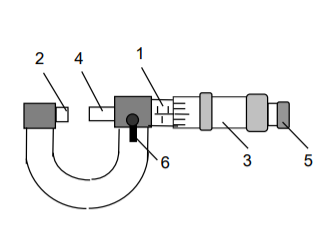
\includegraphics[width=0.4\textwidth]{figures/micrometer.png}
    \captionsetup{justification=raggedright}
    \caption{Micrometer}
    \label{fig:micrometer}
\end{wrapfigure}
Accuracy of lace step, flatness and smoothness of the fang bolt head 4 and the fixed head 2, is the determining factor of precision Panme. To avoid damaging the lace system, other Micrometer is added a sliding spindle 5 attached to the tail of the round ruler 3. When the screw turn out, rolling the round ruler 3, when we turn in, rolling the sliding spindle 5, until the fang bolt 4 touch the materials that need to measure, induce the sound crackle. \par
A small lever grip 6 for fixing the fang bolt 4; when measuring, remember to move the grip to the right, so that can rolling the round ruler. \par
Before the test point "0" of Micrometer should be check. Use clean cloth lightly wipe the head face the fixed head 2 and fang bolt 4 (2 faces are polished like mirrors), turn slowly spindle 5 until heard the sound crackles. Observe the bar "0" on round ruler 3. If Micrometer has been adjusted correctly, the bar "0" on the round ruler 3 is coincide with the standard line in screw body 1. In case the baseline is not coincide, asking the instructor to adjust, or record the deviation "0" for later additions. If bar "0" is below the standard, the measurement results must subtract 0,01n (mm) and vice versa. \par
To measure the diameter d of steel balls, put up the steel balls against the fixed head 2, and then slowly turn the screw head 5 to fang bolt 4 enters into contact with steel balls until you hear a crackle than stopped, move the grip 6 to the left side to inhibit the fang bolt 4.
\begin{itemize}
    \item If the edge of the round ruler is closed to the right size of N of integer line (above the baseline) of the double ruler, also the standard line is coincides with m in round ruler, than the diameter of the ball: $d = N + 0.01 \cdot m ~(mm)$
    \item If the edge of the round ruler is closed to the right size of N of semi-integer line (under the baseline) of the double ruler, also the standard line is coincides with m in round ruler, than the diameter of the ball: $d=N' + 0.01 \cdot m = N + 0.5 + 0.01 \cdot m \ (mm)$, where N is the integer line (above range) is located adjacent the left of N'. In other words, $d = 0,5k + 0,01\cdot m$ (k is the total number of line that appear on the edges of round ruler, do not count line 0)
\end{itemize}


\paragraph{Use Micrometer, perform five times the measurements of diameter d, recorded in table (\ref{table:1})}.

\subsubsection{Measure the time interval  of steel balls falling in liquids}
\paragraph{Installation and adjustment of balance.}
\begin{itemize}
    \item Drive the screws on the bottom of the box 8 (Figure 3) to adjust so that the glass tube 2 containing the liquid is vertical direction. Maintaining the head of the sensor 4 and 5 along the bottom of the tube about 30 centimeters apart.
    \item Plug the power grab of the physical device MN-971A into a power ~ 220V. Press the K key on the machine: LED lights glow and the digits displayed in the window "TIME" and "N" on the machine. 
\end{itemize}
\begin{figure}[H]
    \centering
    \captionsetup{justification=centering}
    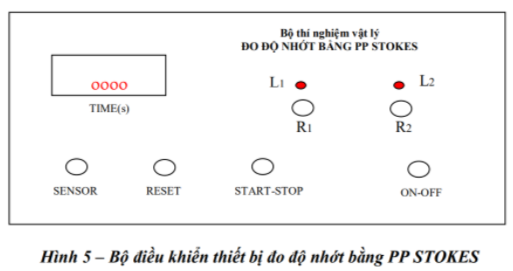
\includegraphics[width=0.6\textwidth]{figures/machine-measure-viscosity.png}
    \caption{The time measurement device used.}
    \label{fig:measurement-device}
\end{figure}

\paragraph{Adjusting the sensitivity of the sensor 4 and 5 of the time measurement device as follows}
\begin{itemize}
    \item Adjusting the sensitivity of the sensor 4 and 5 of the time measurement device as follows
    \item Adjust the sensitivity of the sensor 5 (at the bottom) by turning the knob 7 slowly, according clockwise to the right until the digits displayed on the window "TIME" began to change status (from standing turn to jump number or vice versa), then stop, then return a little to the left (about 1/3- 1/2 of its division). Need to repeat several times to find the exact location of the knob threshold M (7), in which the counter flip status, to be able to put it in position close to the left point M, sensitive enough to the ball passing sensor 5, timer must turn over. This location can verify by tapping the ball into the face of the sensor 5 wall damage: if the digits displayed on the window "TIME" change status 5 status, the sensor has been adjusted sensitive enough to operate.
    \item Perform the same movement for the knob 6 to adjust the sensitivity of the sensor 4 (above). 
    \item Finally click "RESET" to put the digits displayed on the windows are back to 0, the system is ready to measure. Note that, we can only adjust status threshold flip for a sensor when the other sensor is located in front of the threshold flip (left point M).
    \item In case not to use the sensor, the measurement device MN-971A can be used as an electronic stopwatch with an accuracy of 10-3 s, layout buttons on the machine lid. Meanwhile the adjustment knob (6), (7) turn to the left end.
\end{itemize}

\paragraph{Measurement falling time of steel balls}
\begin{itemize}
    \item Slight drop steel balls through hopper to fall vertically along the axis of the glass tube containing the liquid. When the ball goes over the cross section of the sensor 4 or 5, it would appear an electrical impulse effects start or stop the timer device. Period of steel balls  falling on the distance L between the two sensors 4 and 5 on the display window TIME. 
    \item Perform this experiment 10 times with the same steel balls chosen. Read and write the value of  in the display window "TIME" with each measurement in Table 1. (To the left of the window "TIME" are displayed "N" to track the operation number of the sensors 4 and 5: each steel balls passing through a sensor, digit displays in the window "N" is increased by one unit).
\end{itemize}

\newpage
\section{Equations}
\begin{formula}
Given $\eta$ is the viscosity coefficient of fluid (kg/m.s), $\rho_1$ and $\rho$ respectively be the bulk density of steel balls and bulk density of liquid, $d$ is the finite diameter of the cylinder containing the liquid, $g$ is the gravitational acceleration, $\tau$ is the time period between two
selected baseline. $L$ is the distance between 2 baselines, $D$ is the diameter of vertical tube:
\[\eta = \frac{1}{18} \frac{(\rho_1 - \rho)\cdot d^2 \cdot g \cdot \tau}{L\left(1+2.4\frac{d}{D}\right)} \]
\end{formula}
\begin{proof}
We have: 
\begin{equation} \label{eqn:1}
F_{ms}=\eta \frac{dv}{dz}\cdot \Delta S
\end{equation}
, in which $F_{ms}$ is the value of internal friction between 2 liquid layers with velocity is $v$ and $v + dv$, is separated by a distance $dz$ along the $Oz$ axis, is proportional to the
gradient velocity following $Oz$ $dv/dz$ and is proportional to the surface area $\Delta S$. \par
Experiment shows on the distance $2r/3$, from the outside
steel balls away, the velocity of the liquid layer decreases from $v$ to 0. Meanwhile the gradient velocity with Oz:
\begin{equation} \label{eqn:2}
    \frac{dv}{dz} = \frac{v-0}{\frac{2r}{3}}= \frac{3v}{2r}
\end{equation}
According to the formula (\ref{eqn:1}), internal friction between adhesive liquid layers on the outer surface of the steel balls, (an area $\Delta S=4\pi r^2$, $r$: radius of steel balls) and the liquid
layers contact with it have value:
\begin{equation} \label{eqn:3}
    F_{ms}=\eta \frac{dv}{dz}\cdot \Delta S = \eta \frac{3v}{2r} 4\pi r^2
\end{equation}
Gravity $P$ vertically from top to bottom and has the value by:
\begin{equation} \label{eqn:4}
    P=mg=\frac{4}{3}\pi r^3 \cdot \rho_1 g
\end{equation}
With $r$ is the radius and $\rho_1$ is the bulk density of steel balls, $g$ is the gravitational acceleration. \par
Acsimet force $F_A$ is vertical direction from the bottom up and has value by the weight of the liquid being occupied by the steel balls:
\begin{equation}\label{eqn:5}
    F_A=\frac{4}{3}\pi r^3 \cdot \rho \cdot g
\end{equation}
With $\rho$ is the bulk density of liquid. \par
The internal friction force $F_C$ is vertically from the bottom up and have value by:
\begin{equation} \label{eqn:6}
    F_C=6\pi \cdot \eta \cdot r \cdot v
\end{equation}
With $v$ is velocity and $eta$ is viscosity coefficient of liquid. \par
Under the effect of the forces mentioned above, marble will move with acceleration: 
\[a=\frac{dv}{dt}\]
following the second Newton laws: 
\begin{equation}\label{eqn:7}
    m\frac{\overrightarrow{dv}}{dt}=\overrightarrow{P} + \overrightarrow{F_A} + \overrightarrow{F_C}
\end{equation}
Give equation (\ref{eqn:7}) is 0 and follow the direction of steel balls motion, we have:
\begin{equation}\label{eqn:8}
    \eta = \frac{2}{9} \frac{(\rho_1 - \rho)\cdot r^2 \cdot g}{v_0}
\end{equation}
$v_0$ can be determined by measuring the number of time interval movement
$\tau$ of steel balls that are falling between two straight baseline 4 and 5 separated by a distance $L$. \par
Subtitute $v_0$ in (\ref{eqn:8}) with d is the diameter of the steel balls, we find:
\begin{equation}\label{eqn:9}
    \eta = \frac{1}{18} \frac{(\rho_1 - \rho)\cdot d^2 \cdot g \cdot \tau}{L}
\end{equation}
In fact, liquid is not infinitely wide, it is contained in a cylinder with a finite diameter $d$. In this case, the viscosity coefficient of the fluid is calculated using the formula:
\begin{equation}
    \eta = \frac{1}{18} \frac{(\rho_1 - \rho)\cdot d^2 \cdot g \cdot \tau}{L\left(1+2.4\frac{d}{D}\right)}
\end{equation}
Our proof done.
\end{proof}


\newpage
\section{Experimental Data}
\begin{table}[h!]
\centering
\begin{tabular}{|p{0.8in}|p{0.9in}|p{0.5in}|p{0.4in}|p{0.9in}|p{0.9in}|} 
\hline 
\multicolumn{3}{|p{3in}|}{
- Accuracy of\newline
+ Caliper: 0.02 (mm) \newline
+ Time meter: 0.001 (s)\newline
- Diameter of vertical tube: \newline
D = 35.00 ${\pm}$ 0.02 (mm)\newline 
- Mass of the marbles: m = 1.04 ${\pm}$ 0.02 (g)
} & \multicolumn{3}{|p{2.3in}|}{
* Density of oil: $\rho $ = 895 ${\pm}$ 89 (kg/m${}^{3}$)  \newline
* Distance: L = 300 ${\pm}$ 1 (mm)
} \\ \hline 
Data & d (mm) & \multicolumn{2}{|p{0.9in}|}{ $\Delta$d (mm)} & $\tau$ (s ) & $\Delta$$\tau$  (s ) \\ \hline 
1 & 6.31 & \multicolumn{2}{|p{0.9in}|}{0.004} & 0.978 & 0.0102 \\ \hline 
2 & 6.32 & \multicolumn{2}{|p{0.9in}|}{0.006} & 0.970 & 0.0022 \\ \hline 
3 & 6.31 & \multicolumn{2}{|p{0.9in}|}{0.004} & 0.955 & 0.0128 \\ \hline 
4 & 6.33 & \multicolumn{2}{|p{0.9in}|}{0.016} & 0.957 & 0.0108 \\ \hline 
5 & 6.30 & \multicolumn{2}{|p{0.9in}|}{0.014} & 0.979 & 0.0112 \\ \hline 
Mean & 6.314 & \multicolumn{2}{|p{0.9in}|}{0.009} & 0.9678 & 0.0094 \\ \hline 
\end{tabular}
\caption{Table of given and experimental measured data.}
\label{table:1}
\end{table}

\[\overline{d} = \frac{6.31 + 6.32 + 6.31 + 6.33 + 6.30}{5} = 6.314\ (mm)\] 
\[\overline{\tau} = \frac{0.978 + 0.970 + 0.955 + 0.957 + 0.979}{5} = 0.9678\ (s)\] 
\[\Delta d_1 = |6.314 - 6.31| = 0.004\ (mm)\]
\[\Delta d_2 = |6.314 - 6.32| = 0.006\ (mm)\]
\[\Delta d_3 = |6.314 - 6.31| = 0.004\ (mm)\]
\[\Delta d_4 = |6.314 - 6.33| = 0.016\ (mm)\]
\[\Delta d_5 = |6.314 - 6.30| = 0.014\ (mm)\]
\[\Delta \overline{d} = \frac{0.004 + 0.006 + 0.004 + 0.016 + 0.014}{5} = 0.009\ (mm)\] 
\[\Delta \tau_1 = |0.9678 - 0.978| = 0.0102\ (s)\]
\[\Delta \tau_2 = |0.9678 - 0.970| = 0.0022\ (s)\]
\[\Delta \tau_3 = |0.9678 - 0.955| = 0.0128\ (s)\]
\[\Delta \tau_4 = |0.9678 - 0.957| = 0.0108\ (s)\]
\[\Delta \tau_5 = |0.9678 - 0.979| = 0.0112\ (s)\]
\[\Delta \overline{\tau} = \frac{0.0102 + 0.0022 + 0.0128 + 0.0108 + 0.0112}{5} = 0.0094\ (s)\] 
\newpage
\section{Calculations}
\noindent $\pi =3.14\ $and $\Delta \pi =0.005$ \par
\noindent $g=9.81\ m/s^2$ and $\Delta g=0.005\ m/s^2$
\paragraph{Calculating the total absolute errors of the measurement of diameter $d$, timer $\tau$, distance $L$}
\[\Delta d=\Delta d_{sys}+\Delta \overline{d}=\mathrm{0.01}+\mathrm{0.009}=0.019\left({10}^{-3}m\right)\] 
\[\Delta \tau =\Delta {\tau }_{sys}+\Delta \overline{\tau }=\mathrm{0.001\ }+\mathrm{0.0094}\mathrm{=0.0104}\left(s\right)\ \] 
\[\Delta L=\Delta L_{sys}+\Delta \overline{L}=1+0=1\left({10}^{-3}m\right)\ \] 
\[\Delta m=\Delta m_{sys}+\Delta \overline{m}=0.02+0=0.02\left({10}^{-3}\ kg\right)\ \] 
\[\mathrm{\Delta }\rho =\Delta {\rho }_{sys}+\Delta \overline{\rho }=89+0=89\ \mathrm{(kg/m^3}\mathrm{)\ }\] 
\[\Delta D=\Delta D_{sys}+\Delta \overline{D}=0.02+0=0.02\ \left({10}^{-3}m\right)\ \] 
\paragraph{Calculating the density of the marble and the relative error}
\[{\overline{\rho_1}}=\dfrac{\overline{m}}{\dfrac{1}{6}\pi \cdot {\overline{d}}^3}=\dfrac{1.04\times {10}^{-3}}{\dfrac{1}{6}\times 3.14\times {\mathrm{(6.314}\times {10}^{-3})}^3}=7894.801(\dfrac{kg}{m^3})\] 
and
\[\dfrac{\Delta {\rho }_1}{{\overline{\rho_1 }}}=\dfrac{\Delta m}{\overline{m}}+\dfrac{\Delta \pi }{\pi }+\dfrac{3\Delta d}{\overline{d}}\]
Then,
\[\Delta {\rho_1}=\left(\dfrac{\Delta m}{\overline{m}}+\dfrac{\Delta \pi }{\pi }+\dfrac{3\Delta d}{\overline{d}}\right)\times {\overline{\rho_1 }}=\ \left(\dfrac{0.02}{1.04}+\dfrac{0.005}{3.14}+\dfrac{3\times 0.019}{\mathrm{6.314}}\right)\times 7894.801=235.665 (\dfrac{kg}{m^3})\]

\paragraph{Calculating the coefficient of viscosity of liquid and the relative error:}
\[\overline{\eta }=\dfrac{1}{18}\times \dfrac{({\overline{\rho }}_1-\overline{\rho }){\overline{d}}^2g\overline{\tau }}{\overline{L}(1+2,4\dfrac{\overline{d}}{\overline{D}})}=\dfrac{1}{18}\times \dfrac{(7894.801-895)\times {\left(6.314\times {10}^{-3}\right)}^2\times 9.81\times 0.9678}{(300\times {10}^{-3})\times (1+2,4\ \times \dfrac{\mathrm{6.314}}{\mathrm{35.00}})}=0.342(\dfrac{kg}{m.s})\]

\[\dfrac{{\Delta}\eta }{\overline{\eta }}=
\dfrac{\Delta \rho_1+ {\Delta }\rho }{{\overline{\rho }}_1-\overline{\rho }}+\dfrac{\mathrm{\Delta }g}{g}+\dfrac{{\Delta}\tau }{\overline{\tau }}+\dfrac{\mathrm{\Delta }L}{\overline{L}}+\dfrac{1}{\overline{D}+2,4\overline{d}} \left[\left(2\overline{D}+2,4\overline{d}\right)\dfrac{\mathrm{\Delta }d}{\overline{d}}+2,4\overline{d}.\dfrac{\mathrm{\Delta }D}{\overline{D}}\right]\]

\[\mathrm{\Delta }\eta =\overline{\eta }\times \left\{\dfrac{\Delta \rho_1+ {\Delta }\rho }{{\overline{\rho }}_1-\overline{\rho }}+\dfrac{\mathrm{\Delta }g}{g}+\dfrac{{\Delta}\tau }{\overline{\tau }}+\dfrac{\mathrm{\Delta }L}{\overline{L}}+\dfrac{1}{\overline{D}+2,4\overline{d}} \left[\left(2\overline{D}+2,4\overline{d}\right)\dfrac{\mathrm{\Delta }d}{\overline{d}}+2,4\overline{d}.\dfrac{\mathrm{\Delta }D}{\overline{D}}\right]\right\}(\dfrac{kg}{m.s})\]
Then:
\[ \] 
\begin{multline*}
    \mathrm{\Delta }\eta =0.342\times \bigg\{\dfrac{273.176+\mathrm{89}}{7894.\ 801-\mathrm{895}}+\dfrac{0.005}{9.81}+\dfrac{\mathrm{0.0104}}{\mathrm{0.9678}}+\dfrac{\mathrm{1}}{300}+\dfrac{1}{\mathrm{35.00}\times {10}^{-3}+2,4\times \mathrm{6.314}\times {10}^{-3}}\times \\
    \left[\left(\mathrm{2}\times \mathrm{35.00}+2.4\times \mathrm{6.314}\right)\times {10}^{-3}\times \dfrac{0.029}{\mathrm{6.314}}+2,4\times \mathrm{6.314}\times {10}^{-3}\times \dfrac{\mathrm{0.02}}{35.00}\right] \bigg\}=0.023(\dfrac{kg}{m.s})
\end{multline*}


\newpage
\section{Conclusions}
\[\eta = (\overline{\eta} \pm \Delta \eta) = 0.342 \pm 0.023 \bigg( \frac{kg}{m \cdot s}\bigg) \]
% ------------------------------------------
% BIBLIOGRAPHY
% ------------------------------------------
% \newpage
% \bibliography{references}

% ------------------------------------------
% APPENDICES & ATTACHMENTS
% ------------------------------------------

\end{document}